\documentclass[12pt]{article}

%-------------PACKAGES------------- 
\usepackage[margin=1in]{geometry} 
\usepackage{amsmath,amsthm,amssymb}
\usepackage{pgfplots}
\usepackage{float}
\usepackage{braket}
\usepackage{titling}
\usepackage{wrapfig}
\usepackage{tikz}
\usepackage{mwe}
\usepackage{mathtools}
\usepackage{scrextend}
\usepackage{listings}
\usepackage{color}
\usepackage{caption}
\usepackage{subcaption}
\usepackage{algorithm,algpseudocode}
\usetikzlibrary{shapes,arrows,chains}
\usetikzlibrary[calc]

%-------------FORMATTING-------------
\setlength{\droptitle}{-7.5em} 
\setlength{\parindent}{0pt}
\def\LW{\dimexpr.25\linewidth-.5em} 
\tikzstyle{line} = [draw, -latex']
 
%--------------COMMANDS--------------
\newcommand{\N}{\mathbb{N}}
\newcommand{\Z}{\mathbb{Z}}
\newcommand{\R}{\mathbb{R}}
\newcommand{\C}{\mathbb{C}}
%\renewcommand{\qedsymbol}{\filledbox}

\DeclarePairedDelimiter \abs{\lvert}{\rvert}%
\DeclarePairedDelimiter \babs{\bigg\lvert}{\bigg\rvert}%
\DeclarePairedDelimiter \norm{\lVert}{\rVert}%

%------------ENVIRONMENTS------------- 
\newenvironment{theorem}[2][]{\begin{trivlist}
\item[{\bfseries #1}\hskip \labelsep {\bfseries #2.}]}{\end{trivlist}}
\newenvironment{lemma}[2][Lemma]{\begin{trivlist}
\item[\hskip \labelsep {\bfseries #1}\hskip \labelsep {\bfseries #2.}]}{\end{trivlist}}
\newenvironment{exercise}[2][Exercise]{\begin{trivlist}
\item[\hskip \labelsep {\bfseries #1}\hskip \labelsep {\bfseries #2.}]}{\end{trivlist}}
\newenvironment{reflection}[2][Reflection]{\begin{trivlist}
\item[\hskip \labelsep {\bfseries #1}\hskip \labelsep {\bfseries #2.}]}{\end{trivlist}}
\newenvironment{proposition}[2][Proposition]{\begin{trivlist}
\item[\hskip \labelsep {\bfseries #1}\hskip \labelsep {\bfseries #2.}]}{\end{trivlist}}
\newenvironment{corollary}[2][Corollary]{\begin{trivlist}
\item[\hskip \labelsep {\bfseries #1}\hskip \labelsep {\bfseries #2.}]}{\end{trivlist}}
\newenvironment{definition}[2][]{\begin{trivlist}
\item[{\bfseries #1}\hskip \labelsep {\bfseries #2.}]}{\end{trivlist}}
\theoremstyle{remark}
\newtheorem*{remark}{Remark}

%-------------CODE-STYLE------------
\definecolor{dkgreen}{rgb}{0,0.6,0}
\definecolor{gray}{rgb}{0.5,0.5,0.5}
\definecolor{mauve}{rgb}{0.58,0,0.82}
\lstset{frame=tb,
	language=C++,
	aboveskip=3mm,
	belowskip=3mm,
	showstringspaces=false,
	columns=flexible,
	basicstyle={\small\ttfamily},
	numbers=none,
	numberstyle=\tiny\color{gray},
	keywordstyle=\color{blue},
	commentstyle=\color{dkgreen},
	stringstyle=\color{mauve},
	breaklines=true,
	breakatwhitespace=true,
	tabsize=3
}

\tikzset{
	path image/.style={
		path picture={
			\node at (path picture bounding box.center) {
				\includegraphics[height=3cm]{example-image}};}},
	path tikzimage/.style={
		path picture={
			\node at (path picture bounding box.center)
			[circle, fill=blue!50, scale=2, text=yellow]{Bravo};}}
}
	
\lstset{
	morekeywords={end}
}

%------------------------------------ 
%---------START-OF-DOCUMENT----------
%------------------------------------
\begin{document}
 
\title{Paper Summary}
\author{David Miller \\ 
CIS 5930: Social Network Mining} 

\maketitle

Deep Learning is a machine learning method based on learning data representations. The main goal of most deep learning systems, or neural networks, is to identify expert neurons and use them for training. Current implementations of neural networks require large matrix multiplications to determine the energy of each neuron, where higher energy can be thought of as an expert neuron. Even when matrices are sparse and clever numerical methods are implemented to compute matrix multiplications, the amount of FLOPS still remains computationally expensive. The paper aims at using a hashing approach to identify expert neurons. 
\begin{wrapfigure}{l}{0.5\textwidth}
	\vspace{-15pt}
	\hspace{-20pt}
	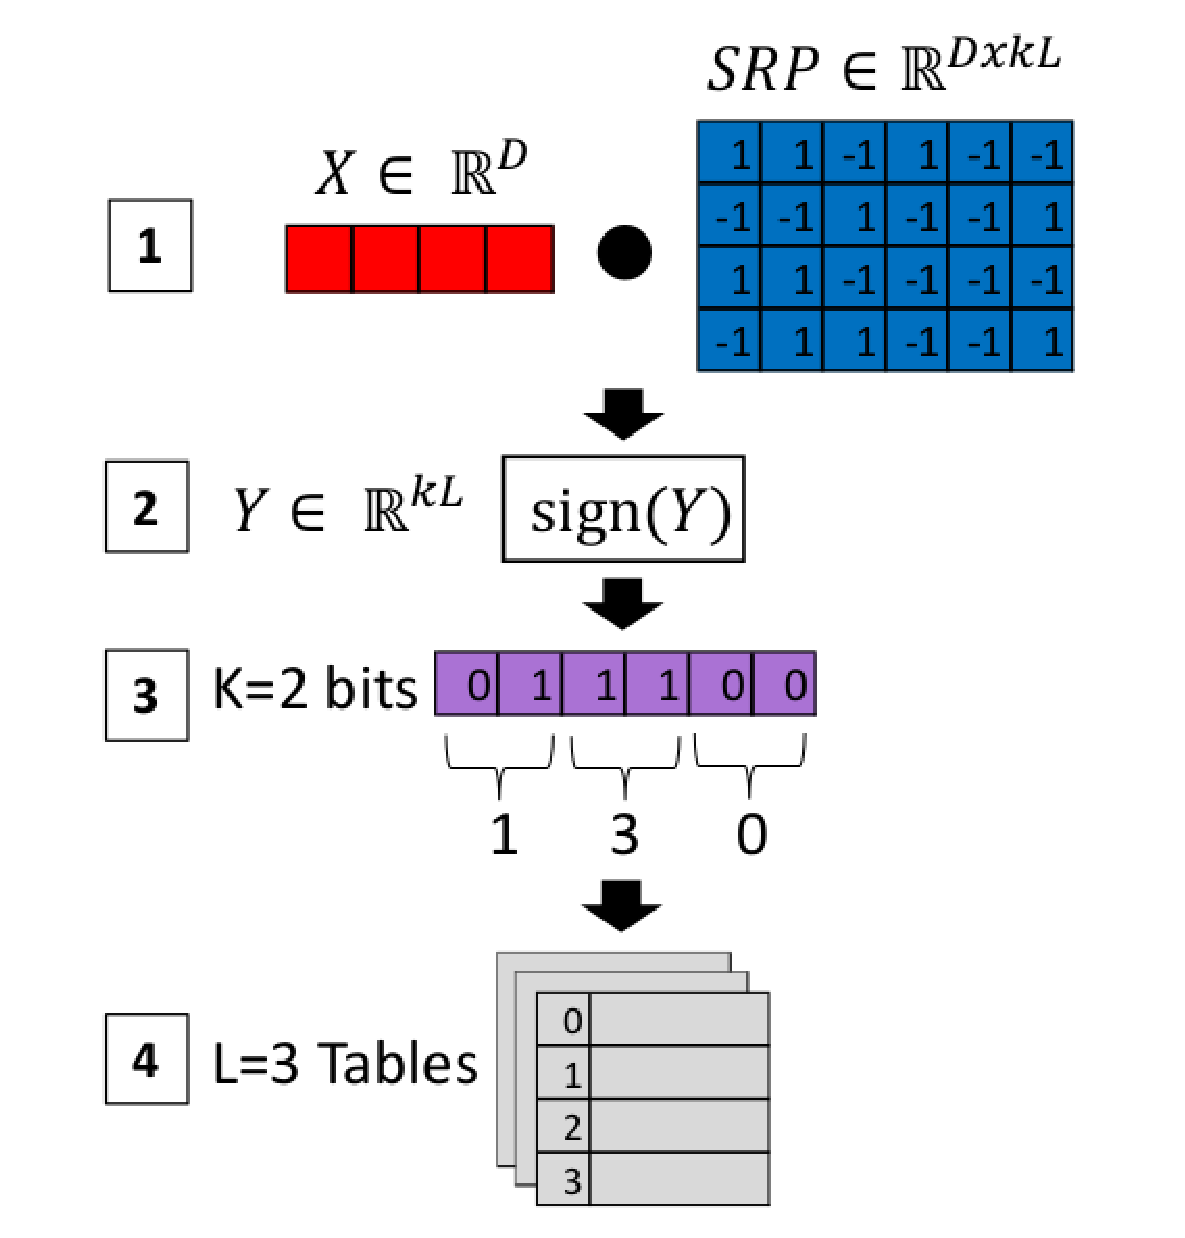
\includegraphics[height=6.5cm,width=0.425\textwidth]{Figure1.eps}
	\caption{}
\end{wrapfigure}
\vspace{-13pt}
\begin{addmargin}[-40.3pt]{0pt}
The first step is to take each element $x \in X \subset \mathbb{R}^D$ and take the inner product with a random signed matrix $SRP \subset \mathbb{R}^{D \times kL}$. From $x \boldsymbol{\cdot} SRP = Y \subset \mathbb{R}^{kL}$ we can perform Hash$_i(Y)$ for $i = 1, ..., k$ to obtains a collection of fingerprints. These fingerprints are used to index into HashTable$_j$ for $j = 1, ..., L$. Figure 1 illustrates the inner product between a data vector and a random SRP and the result being hashed on by the signum function to index into three HashTables. Each entry in a HashTable is called a bucket since they hold onto multiple neurons. The final step is to then union a bucket from each HashTable, where these buckets will be the expert neurons. Therefore we get that the output at each layer is Bucket$_1 \cup \dots \cup$ Bucket$_L$ where Bucket$_j \in $ HashTable$_j$. However
\end{addmargin}
keeping multiple HashTables can be taxing on the memory so the paper uses multi-probe Local Sensitive Hashing (LSH). Rather than have $L$ HashTables and take a single bucket from each, multi-probe LSH constructs only $L^\prime < L$ HashTables and takes multiple buckets per HashTable. The other buckets are ones that are neighbors to that 
\begin{wrapfigure}{r}{0.5\textwidth}
	\vspace{-15pt}
	\hspace{0pt}
	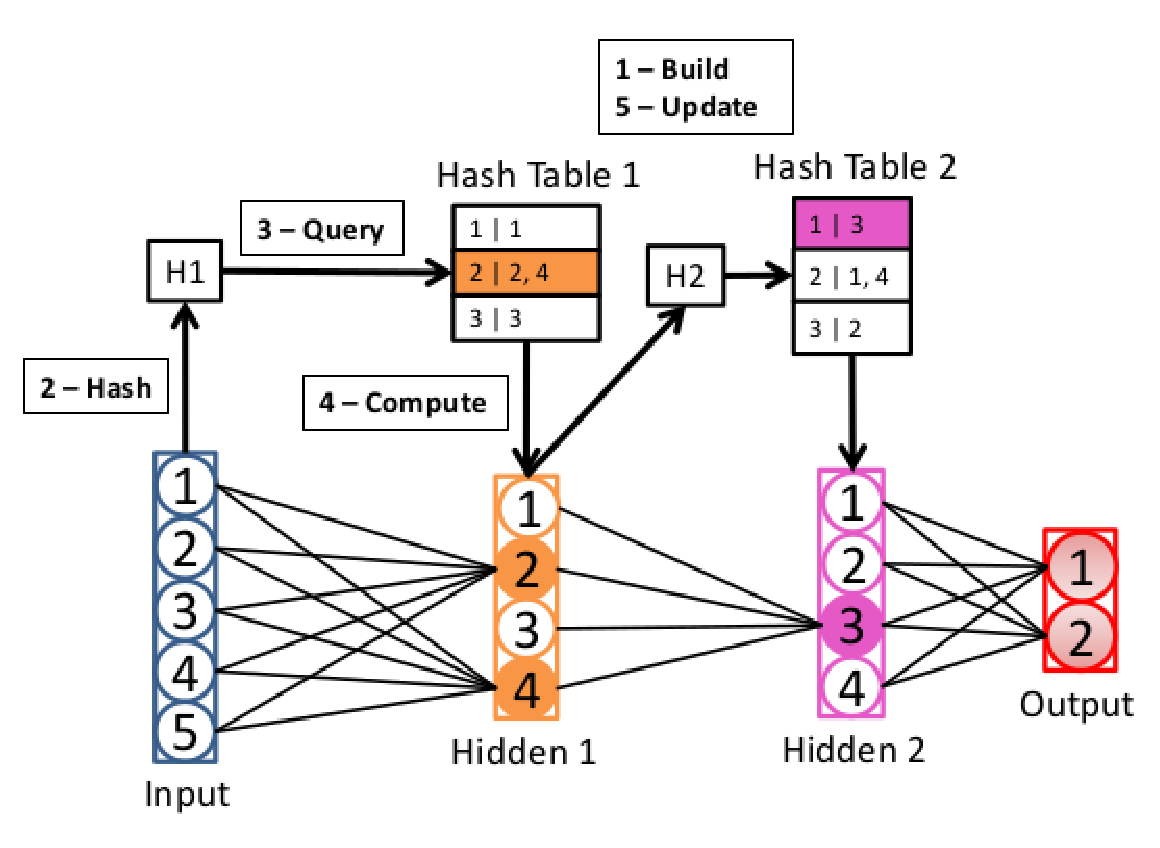
\includegraphics[height=5.25cm,width=0.5\textwidth]{Figure2.eps}
	\caption{}
	\vspace{-20pt}
\end{wrapfigure}
of the primary bucket, that is the buckets have neurons that are close to the energy of the primary bucket. Therefore the output now becomes Bucket$_1^1 \cup ... \cup$ Bucket$_1^n \cup ... \cup$ Bucket$_{L^\prime}^1 \cup ... \cup$ Bucket$_{L^\prime}^n$ where Bucket$_j^m$ is the $m$-th Bucket for HashTable$_j$. Figure 2 illustrates five inputs (data vectors that have taken the inner product with some SRP) being hashed on by some arbitrary hash function H1 and indexed into the first HashTable. At the same time, the same input data is hashed on by another arbitrary hash function H2 and indexed into the second hash table. The output is the union of buckets of expert neurons, in this case it is Bucket$_2$ from the first HashTable and Bucket$_1$ from the second HashTable. In terms of future work, the section provided in the paper discusses the most used technology in today's world: mobile processing. Due to the efficiency and lightweight framework of the method presented in this paper, optimization for mobile processors should not present to big of a problem. Since essentially everyone owns a phone, each person will act as a contributor to a huge mobile processor cluster. Anotehr direction that can be taken in the future is warehouse scale computing. The savings in computational time allows warehouse scale computing to perform an enormous amount of parallel deep learning tasks. \\

In terms of strengths of the paper, there are three that stand out to me
\begin{enumerate}
	\item The method presented in the paper achieves an average of 99\% accuracy compared to classical deep learning methods while using significantly less neurons.
	\item The method presented in the paper is a lightweight framework due to it uses pointers to its data rather than storing it in memory.
	\item The time complexity of the method presented in the paper is at worst $\mathcal{O}(n)$ at each layer due to the efficiency of hash tables.
\end{enumerate}

There are not three strong flaws in the paper I could find but there were definitely ones that can be further analyzed 
\begin{enumerate}
	\item Due to the nature of Hash Tables there is no efficient way to identify neighbors of the primary bucket, therefore multi-probe LSH might present some computational complexity problems.
	\item Statistically there is a small chance that most of the neurons can be put into the same bucket and therefore the output will have almost the same amount of neurons that was present initially.
	\item Since the method is heavily reliant on statistical methods, a large data set is required to achieve accurate results.
\end{enumerate}

Questions for the presenter
\begin{enumerate}
	\item How are $k$, $L$, and buckets per table determined? 
	\item Is there an analysis that can be done on the choice of $k$, $L$, and buckets per table that can tell us how "good" the results will be?
	\item Is there a way for the user to assign a matrix rather than some $SRP$, and if so does it have to be a matrix such that each entry is in $[-1,1]$?
\end{enumerate}

\end{document}